% !TeX program = xelatex
\documentclass[aspectratio=169,11pt]{beamer}
% Shared preamble of the three slide decks of this unit
% (slides_lm1.tex, slides_lm2.tex, slides_lm3.tex).
% The look is the same as the PINN and CNN slides.
% The figure files in tikz/ are the ones of the notes (main.tex),
% so the colors and TikZ styles below are the same as in the notes.

% -------------------------------------------------
% Packages
% -------------------------------------------------
\usepackage{kotex}
\usepackage{fontspec}
\usepackage{amsmath,amssymb,bm,mathtools}
\usepackage{booktabs,array}
\usepackage{xcolor}
\usepackage{colortbl}
\usepackage{tikz}
\usetikzlibrary{positioning,arrows.meta,calc,fit,backgrounds,
  decorations.pathreplacing,shapes.misc}
\usepackage[most]{tcolorbox}
\usepackage{listings}
\usepackage{adjustbox}

% -------------------------------------------------
% Colors (same as the notes)
% -------------------------------------------------
\definecolor{deepblue}{RGB}{34,71,120}
\definecolor{softblue}{RGB}{239,246,253}
\definecolor{softgray}{RGB}{246,247,249}
\definecolor{softgreen}{RGB}{239,249,242}
\definecolor{softyellow}{RGB}{255,249,229}
\definecolor{codegray}{RGB}{248,248,248}
% colors of the figures
\definecolor{tokc}{RGB}{31,100,180}
\definecolor{hotc}{RGB}{200,30,40}
\definecolor{attc}{RGB}{214,110,0}
\definecolor{grnc}{RGB}{40,140,70}

% TikZ styles used by the files in tikz/ (same as the notes)
\tikzset{
  >=Latex,
  tok/.style={draw=#1!70!black,fill=#1!10,rounded corners=2pt,font=\ttfamily,
    minimum height=7mm,inner sep=3pt},
  tok/.default=tokc,
  lay/.style={draw=#1!70!black,fill=#1!8,rounded corners=3pt,align=center,
    minimum height=8mm,minimum width=22mm,inner sep=3pt},
  lay/.default=black,
  neu/.style={circle,draw=black!70,minimum size=5.5mm,inner sep=0pt,font=\small},
  ar/.style={->,thick,#1},
  ar/.default=black!80,
  op/.style={circle,draw,inner sep=1pt,minimum size=6mm,font=\small},
  lab/.style={font=\small,align=center},
}

% -------------------------------------------------
% Beamer look (same as the PINN and CNN slides)
% -------------------------------------------------
\usetheme{default}
\usefonttheme[onlymath]{serif}
\setbeamertemplate{navigation symbols}{}
\setbeamersize{text margin left=8mm,text margin right=8mm}
\setbeamercolor{structure}{fg=deepblue}
\setbeamercolor{frametitle}{fg=deepblue}
\setbeamercolor{title}{fg=deepblue}
\setbeamerfont{frametitle}{size=\large,series=\bfseries}
\setbeamertemplate{itemize items}[circle]
\setbeamertemplate{enumerate items}[default]
\setbeamertemplate{frametitle}{%
  \vskip3mm
  {\usebeamerfont{frametitle}\usebeamercolor[fg]{frametitle}\insertframetitle\par}%
  \vskip1mm
  {\color{deepblue!45}\hrule height 0.6pt}%
  \vskip1mm}
\setbeamertemplate{footline}{%
  \hbox to\paperwidth{%
    \hspace*{8mm}{\color{black!45}\scriptsize \insertshorttitle
      \ifx\insertsectionhead\empty\else\ \ $\cdot$\ \ \insertsectionhead\fi}%
    \hfill{\color{black!45}\scriptsize\insertframenumber\,/\,\inserttotalframenumber}%
    \hspace*{8mm}}%
  \vskip2.5mm}
\setbeamertemplate{title page}{%
  \vfill
  \begin{center}
  {\color{deepblue}\Huge\bfseries\inserttitle\par}
  \vskip3mm
  {\color{deepblue!60}\rule{9cm}{0.8pt}\par}
  \vskip3mm
  {\large\insertsubtitle\par}
  \vskip8mm
  {\normalsize\insertdate\par}
  \end{center}
  \vfill}
\AtBeginSection[]{%
  \begin{frame}
  \vfill
  \centering
  {\color{deepblue!55}\Large\bfseries \insertsectionnumber\par}
  \vskip2mm
  {\color{deepblue}\LARGE\bfseries\insertsectionhead\par}
  \vskip3mm
  {\color{deepblue!50}\rule{7cm}{0.8pt}\par}
  \vfill
  \end{frame}}
\setlength{\leftmargini}{1.2em}
\setlength{\leftmarginii}{1.1em}
% numbered sections in the table of contents. The second and third decks start at
% section 5 and 9 like the notes: \setcounter{section}{4} before the first \section,
% and \tableofcontents[firstsection=-3] (third deck: -7) so that the list shows 5-8 (9-11).
\setbeamertemplate{section in toc}[sections numbered]

% -------------------------------------------------
% Boxes (same colors as the notes). The title is braced, so it may contain commas.
% -------------------------------------------------
\newtcolorbox{keybox}[1][]{colback=softblue,colframe=deepblue,boxrule=0.7pt,arc=2mm,
  title={#1},fonttitle=\bfseries\small,left=2mm,right=2mm,top=1mm,bottom=1mm,
  toptitle=0.5mm,bottomtitle=0.5mm}
\newtcolorbox{thinkbox}[1][]{colback=softyellow,colframe=orange!70!black,boxrule=0.6pt,
  arc=2mm,title={#1},fonttitle=\bfseries\small,left=2mm,right=2mm,top=1mm,bottom=1mm,
  toptitle=0.5mm,bottomtitle=0.5mm}
\newtcolorbox{remarkbox}[1][]{colback=softgray,colframe=black!45,boxrule=0.5pt,arc=2mm,
  title={#1},fonttitle=\bfseries\small,left=2mm,right=2mm,top=1mm,bottom=1mm,
  toptitle=0.5mm,bottomtitle=0.5mm}
\newtcolorbox{mlbox}[1][]{colback=softgreen,colframe=green!45!black,boxrule=0.6pt,
  arc=2mm,title={#1},fonttitle=\bfseries\small,left=2mm,right=2mm,top=1mm,bottom=1mm,
  toptitle=0.5mm,bottomtitle=0.5mm}

% -------------------------------------------------
% Code style
% -------------------------------------------------
\lstdefinestyle{pythonstyle}{
  language=Python,
  backgroundcolor=\color{codegray},
  basicstyle=\ttfamily\scriptsize,
  keywordstyle=\bfseries\color{deepblue},
  commentstyle=\itshape\color{black!55},
  stringstyle=\color{black!75},
  numbers=none,
  frame=single,
  rulecolor=\color{black!25},
  breaklines=true,
  showstringspaces=false,
  tabsize=4,
  columns=fullflexible,
  keepspaces=true,
  aboveskip=1mm,
  belowskip=1mm
}
\lstset{style=pythonstyle}

% -------------------------------------------------
% Math commands (same as the notes)
% -------------------------------------------------
\newcommand{\R}{\mathbb{R}}
\newcommand{\vect}[1]{\bm{#1}}
\newcommand{\T}{^{\mathsf T}}
\newcommand{\loss}{\mathcal{L}}
\newcommand{\softmax}{\operatorname{softmax}}
\newcommand{\w}[1]{\texttt{#1}}

% -------------------------------------------------
% Figures
% -------------------------------------------------
% one-line caption under a figure
\newcommand{\figcap}[1]{\par\vskip1mm{\centering\footnotesize\color{black!70}#1\par}}
% TikZ figure of the notes, shrunk to fit: \sfig[max height]{file name in tikz/}
\newcommand{\sfig}[2][5.4cm]{%
  \par{\centering
  \begin{adjustbox}{max width=\linewidth,max totalheight=#1}\input{tikz/#2}\end{adjustbox}
  \par}}
% picture from figures/, fit into the given height: \pfig[max height]{file}
\newcommand{\pfig}[2][5.4cm]{%
  \par{\centering
  \includegraphics[width=\linewidth,height=#1,keepaspectratio]{#2}\par}}


% Used only in this deck.
% Attention weights of the, cat, sat at the position of sat, drawn as bars:
% \wbars{weight of the}{weight of cat}{weight of sat}
\newcommand{\wbars}[3]{%
  \begin{tikzpicture}[x=10mm,y=26mm]
  \foreach \wa/\wn/\wi in {#1/the/0,#2/cat/1,#3/sat/2}{
    \fill[attc!75] (\wi-0.3,0) rectangle (\wi+0.3,\wa);
    \node[font=\scriptsize,above] at (\wi,\wa) {\wa};
    \node[font=\ttfamily\small,below] at (\wi,0) {\wn};
  }
  \draw[black!50] (-0.6,0) -- (2.6,0);
  \node[font=\scriptsize] at (1,1.18) {weights at \texttt{sat}};
  \end{tikzpicture}}

\title[자연어 처리와 언어모델]{자연어 처리와 언어모델}
\subtitle{필요한 곳을 찾아 보기: 어텐션과 Transformer (9--11절)}
\date{딥러닝개론및연습 $\cdot$ 2026년 2학기}

\begin{document}

% =================================================
\begin{frame}[plain]\titlepage\end{frame}

\begin{frame}{복습: 문장을 다루는 신경망 (5--8절)}
\begin{itemize}
\item \textbf{언어모델}: 앞의 단어들로 다음 단어의 확률을 계산한다.
  성능은 퍼플렉서티로 잰다.
\item \textbf{RNN}: 은닉 상태 $\vect h_t$에 지금까지의 단어를 요약하며 한 단어씩 읽는다.
\item \textbf{LSTM}: 기억 셀 $\vect c$와 세 게이트로 먼 과거까지 gradient를 전달한다.
  PTB 테스트 퍼플렉서티는 RNN $161.9$, LSTM $144.3$.
\item \textbf{문장 생성}: 확률분포에서 단어를 뽑아 다음 입력으로 넣기를 반복한다.
\item \textbf{seq2seq}: Encoder가 입력을 벡터 $\vect h$로 요약하고,
  Decoder가 $\vect h$에서 출력 문장을 만든다.
\end{itemize}
\vskip1mm
\begin{remarkbox}[남은 문제]
Encoder는 입력 문장이 아무리 길어도 \textbf{고정 길이 벡터 $\vect h$ 하나}로 요약한다.
엿보기 (peeky)는 $\vect h$를 여러 번 보게 했을 뿐, $\vect h$ 자체의 크기는 그대로이다.
\end{remarkbox}
\end{frame}

\begin{frame}{여기서 다룰 질문}
\begin{keybox}[여기서 다룰 질문]
\begin{itemize}
\item 번역문의 단어를 하나 쓸 때마다
  \textbf{입력 문장의 필요한 부분을 직접 찾아 보게} 할 수 없을까?
  \hfill $\to$ 어텐션
\item RNN은 한 단어씩 순서대로 계산한다.
  RNN 없이 \textbf{어텐션만으로} 문장을 읽을 수 있을까?
  \hfill $\to$ Transformer
\item 그렇게 만든 언어모델은 RNN, LSTM 언어모델과 무엇이 다른가?
  지금의 대화형 언어모델과는?
  \hfill $\to$ GPT
\end{itemize}
\end{keybox}
\vskip2mm
8절의 seq2seq에서 출발해, 지금의 언어모델 (GPT 등)의 핵심인 어텐션과 Transformer까지 간다.
\end{frame}

\begin{frame}{학습목표}
\begin{enumerate}
\item 고정 길이 벡터의 한계와, 어텐션이 그것을 푸는 방법: 내적, softmax, 가중합
\item 어텐션을 넣은 seq2seq의 구조와 구현, 날짜 변환에서 어텐션 가중치 읽기
\item self-attention을 작은 예 (\w{the cat sat})로 한 단계씩 만들기:
  query, key, value, $\sqrt d$로 나누는 이유
\item causal mask, 위치 벡터, multi-head attention,
  Transformer 블록 (Feed Forward, residual 연결, LayerNorm)
\item GPT: Decoder 블록만 쌓은 언어모델의 구현과 PTB에서 RNN, LSTM과의 비교
\item 고정된 단어 벡터와 문맥 표현, 토큰과 BPE
\item 작은 GPT에서 대화형 언어모델로: 크기, 학습 단계, 최근의 흐름
\end{enumerate}
\end{frame}

% firstsection=-7: the TOC counts this deck's sections 1, 2, 3; show them as 9, 10, 11
\begin{frame}{목차}
\tableofcontents[firstsection=-7,hideallsubsections]
\end{frame}

% sections are numbered 9-11 as in the notes
\setcounter{section}{8}

% =================================================
\section{어텐션}
% =================================================

\subsection{고정 길이 벡터의 한계}

\begin{frame}{고정 길이 벡터의 한계}
seq2seq의 Encoder는 입력 문장의 길이와 상관없이 같은 크기의 벡터 $\vect h$ 하나를 낸다.
\sfig[2.6cm]{fixed_len}
\figcap{짧은 문장도 긴 문장도 같은 크기의 벡터 하나로 요약된다.}
\vskip2mm
긴 문장의 정보를 작은 벡터 하나에 다 담기는 어렵다.
\vskip1mm
\begin{keybox}
사람은 원문 전체를 외운 뒤 번역하지 않는다.
번역문의 단어를 하나 쓸 때마다 원문의 \textbf{해당하는 부분을 다시 본다}.
이것을 신경망에서 하는 방법이 \textbf{어텐션} (attention)이다 (Bahdanau et al., 2015).
\end{keybox}
\end{frame}

\subsection{Encoder: 모든 시각의 은닉 상태를 넘긴다}

\begin{frame}{Encoder: 모든 시각의 은닉 상태를 넘긴다}
지금까지는 Encoder의 \textbf{마지막} 은닉 상태만 썼다.
이제 \textbf{모든 시각}의 은닉 상태를 행으로 쌓아 Decoder에 넘긴다.
\sfig[3.2cm]{hs}
\figcap{단어가 $T$개이면 $\vect{hs}$는 $T\times H$ 행렬이다.
  행마다 그 시각의 단어가 대응한다.}
\begin{itemize}
\item 각 행은 그 시각까지 읽은 단어들의 정보를 담지만,
  특히 \textbf{그 시각에 읽은 단어}의 정보를 많이 담는다.
\item 그래서 $\vect{hs}$의 행을 ``입력의 각 단어에 해당하는 벡터''로 본다.
  입력이 길면 $\vect{hs}$도 길어지므로 고정 길이의 제약이 없다.
\end{itemize}
\end{frame}

\subsection{Decoder: 필요한 단어를 골라 본다}

\begin{frame}{Decoder: 필요한 단어를 골라 본다}
\w{I am a cat}을 \w{Je suis un chat}으로 번역할 때
\begin{itemize}
\item \w{Je}를 출력하려면 원문의 \w{I}를, \w{chat}을 출력하려면 \w{cat}을 보아야 한다.
\item 출력할 단어마다 \textbf{입력의 어느 단어를 볼지 고르는} 일을 Decoder에 시킨다.
\end{itemize}
\vskip1mm
\begin{thinkbox}[하나를 고르면 안 되는 이유]
``하나를 고르는'' 연산은 미분할 수 없다. 그래서 역전파로 학습할 수 없다.
\end{thinkbox}
\vskip1mm
그래서 하나를 고르는 대신 모든 단어에 \textbf{가중치} $a_1,\dots,a_T$
($0$ 이상, 합이 $1$)를 주고 가중합을 한다:
\[
\vect c=\sum_{j=1}^T a_j\,\vect{hs}_j .
\]
$\vect c$를 \textbf{맥락 벡터}라 한다.
\end{frame}

\begin{frame}{맥락 벡터: 가중합으로 고르기}
\sfig[4.4cm]{weighted_sum}
\figcap{가중치 $\vect a$로 $\vect{hs}$의 행들을 가중합하여 맥락 벡터 $\vect c$를 만든다.}
\vskip2mm
\begin{keybox}
\w{cat}의 가중치가 $0.8$이면 $\vect c$는 거의 \w{cat}의 벡터가 된다.
사실상 \w{cat}을 고른 것이다.
가중합은 미분할 수 있으므로, 어디에 가중치를 줄지도 역전파로 학습된다.
\end{keybox}
\end{frame}

\subsection{가중치는 어떻게 정하는가}

\begin{frame}{가중치: 내적과 softmax}
가중치는 Decoder의 지금 은닉 상태 $\vect h$와 $\vect{hs}$의 각 행이
얼마나 ``비슷한가''로 정한다. 비슷함은 \textbf{내적}으로 잰다:
\[
s_j=\vect h\cdot\vect{hs}_j\quad(j=1,\dots,T),\qquad \vect a=\softmax(\vect s).
\]
\sfig[3.6cm]{attn_dot}
\figcap{Decoder의 은닉 상태 $\vect h$와 $\vect{hs}$의 각 행의 내적으로 점수 $\vect s$를 계산한다.}
\end{frame}

\begin{frame}{점수에서 가중치로}
\pfig[3.9cm]{figures/attention_softmax.png}
\figcap{점수 $\vect s=(0.5,\ 0.5,\ 1.2,\ 3.3)$에 softmax를 취해
  가중치 $\vect a=(0.05,\ 0.05,\ 0.10,\ 0.80)$를 만든다 (설명을 위해 정한 숫자).}
\vskip1mm
\begin{itemize}
\item softmax 덕분에 가중치는 $0$ 이상이고 합이 $1$이다.
  점수가 가장 큰 \w{cat}이 가중치의 대부분을 받는다.
\item 어떤 단어를 보아야 하는지는 따로 가르치지 않는다.
  번역을 잘하도록 학습하면 $\vect h$와 $\vect{hs}$가
  ``필요한 단어끼리 내적이 크도록'' 만들어진다.
\end{itemize}
\end{frame}

\subsection{어텐션을 넣은 seq2seq}

\begin{frame}{어텐션 계층}
\begin{columns}[c,onlytextwidth]
\begin{column}{0.56\textwidth}
\sfig[6.0cm]{attn_layer}
\end{column}
\begin{column}{0.41\textwidth}
두 단계를 묶은 것이 어텐션 계층이다.
\begin{enumerate}
\item 가중치: $s_j=\vect h\cdot\vect{hs}_j$,\ \ $\vect a=\softmax(\vect s)$
\item 가중합: $\vect c=\sum_j a_j\vect{hs}_j$
\end{enumerate}
\vskip2mm
입력은 Decoder의 $\vect h$와 Encoder의 $\vect{hs}$, 출력은 맥락 벡터 $\vect c$이다.
\vskip2mm
\begin{remarkbox}
이 계층에는 학습되는 가중치가 없다.
학습되는 것은 $\vect h$와 $\vect{hs}$를 만드는 LSTM이다.
\end{remarkbox}
\end{column}
\end{columns}
\end{frame}

\begin{frame}{어텐션을 넣은 seq2seq}
\sfig[5.2cm]{attn_seq2seq}
\figcap{Decoder의 매 시각에 어텐션 계층 (Attn)이 $\vect h$와 $\vect{hs}$에서
  맥락 벡터 $\vect c$를 만들고, Affine은 $\vect c$와 $\vect h$를 함께 받는다.
  주황색 굵은 선은 $\vect{hs}$가 모든 어텐션 계층에 전달되는 것을 나타낸다.}
\end{frame}

\begin{frame}[fragile]{PyTorch로 구현하기 (\texttt{attention\_date.py})}
\texttt{decode} 메서드에서 어텐션에 해당하는 줄들이다.
Decoder의 모든 시각을 한꺼번에 계산하므로, 내적과 가중합이 행렬 곱이 된다.
\begin{lstlisting}
h, state = self.decoder(e, state)     # (B, t, H): decoder hidden states
s = h @ hs.transpose(1, 2)            # (B, t, T): scores h_t . hs_j
a = torch.softmax(s, dim=2)           # attention weights, each row sums to 1
c = a @ hs                            # (B, t, H): context vectors
logits = self.out(torch.cat([c, h], dim=2))
\end{lstlisting}
\begin{itemize}
\item \texttt{h @ hs.transpose(1, 2)}: Decoder의 모든 시각 $t$와 입력의 모든 위치 $j$의
  내적 $\vect h_t\cdot\vect{hs}_j$를 한 번에 계산한다.
\item \texttt{softmax(s, dim=2)}: 입력 위치 방향으로 softmax.
  출력 시각마다 가중치의 합이 $1$이다.
\item \texttt{a @ hs}: 가중합.
  마지막 줄에서 $\vect c$와 $\vect h$를 이어 붙여 Affine 층 (\texttt{self.out})에 넣는다.
\end{itemize}
\end{frame}

\subsection{예: 날짜 형식 바꾸기}

\begin{frame}{예: 날짜 형식 바꾸기}
여러 형식으로 쓴 날짜를 \w{YYYY-MM-DD} 형식으로 바꾼다.
\sfig[2.7cm]{dates}
\begin{itemize}
\item 입력 형식이 다양하다: \w{1994-09-27}의 \w{09}는 \w{september}에서 와야 한다.
  입력과 출력의 대응이 분명해서 어텐션이 무엇을 보는지 확인하기 좋다.
\item 1970년 1월 1일부터 $20{,}001$일 가운데 $2{,}000$일을 테스트용으로 떼어 놓고,
  학습용 예 $45{,}000$개, 테스트용 예 $5{,}000$개를 만든다.
  형식은 다섯 가지, 대소문자도 무작위로 바꾼다.
\item 테스트에 나오는 날짜는 학습 데이터에 어떤 형식으로도 나오지 않는다.
\end{itemize}
\end{frame}

\begin{frame}{결과: 엿보기 seq2seq와 어텐션 seq2seq}
글자 Embedding $16$차원, LSTM $256$차원, 입력 뒤집기, Adam, $10$ epoch.
비교 대상은 8절의 엿보기 seq2seq이다.
\vskip1mm
\begin{columns}[c,onlytextwidth]
\begin{column}{0.47\textwidth}
\pfig[4.6cm]{figures/attention_date_accuracy.png}
\end{column}
\begin{column}{0.5\textwidth}
\small
\begin{tabular}{@{}lcccc@{}}
\toprule
epoch & $1$ & $2$ & $3$ & $10$ \\
\midrule
엿보기 & $0.006$ & $0.568$ & $0.981$ & $1.000$ \\
어텐션 & $0.750$ & $0.985$ & $0.996$ & $0.999$ \\
\bottomrule
\end{tabular}
\vskip1mm
{\footnotesize 테스트 정확도 (답 전체가 맞은 비율)\par}
\vskip3mm
두 모델 모두 결국 거의 다 맞힌다. 차이는 \textbf{빠르기}이다.
어텐션 모델은 1 epoch 만에 $75\%$, 2 epoch 만에 $98.5\%$를 맞혔다.
\end{column}
\end{columns}
\end{frame}

\begin{frame}{어텐션 가중치를 그려 보면}
문제 \w{THURSDAY, JULY 1, 1993}, 답 \w{1993-07-01} (\texttt{attention\_date.py}의 4번 셀)
\pfig[5.3cm]{figures/attention_date_map.png}
\figcap{행은 출력 글자, 열은 입력 글자이다. 색이 진할수록 가중치가 크다.}
\end{frame}

\begin{frame}{어텐션은 무엇을 보았나}
\small
\begin{itemize}
\item 연도 \w{1993}의 각 숫자는 입력의 \w{1993}의 같은 자리를 본다
  (가중치 $1.00$, $0.98$, $0.83$, $1.00$).
\item 월의 \w{7}은 \w{JULY}의 \w{U}를 본다 ($1.00$).
  입력을 뒤집어 넣었으므로 \w{U} 위치의 은닉 상태는 \w{ULY}까지 읽은 요약이다.
  여기서 몇 월인지 알 수 있다.
\item 일의 \w{0}은 \w{1} 앞의 공백을, \w{1}은 입력의 \w{1}을 본다 (둘 다 $1.00$).
  공백 위치에서 날짜가 한 자리 수임을 알 수 있다.
\item \w{-}의 행은 비어 있다. \w{-}는 입력과 상관없이 정해지므로 날짜의 어느 글자도
  볼 필요가 없다 (가중치는 문제 뒤에 채운 공백에 있다: $0.99$, $0.96$).
\item 요일은 답에 필요 없고, 실제로 거의 보지 않는다.
  예외는 월의 \w{0}이 \w{A}에 준 $0.37$이고, 이때도 가중치의 $0.57$은 공백에 있다.
\end{itemize}
\begin{keybox}
무엇을 보아야 하는지는 아무도 알려 주지 않았다.
출력을 맞히도록 학습했을 뿐인데, 출력과 입력의 대응 관계를 스스로 찾았다.
다만 월의 \w{0}처럼 사람이 기대한 곳을 보지 않는 경우도 있다.
\end{keybox}
\end{frame}

\subsection{더 나은 어텐션 seq2seq}

\begin{frame}{더 나은 어텐션 seq2seq}
\textbf{양방향 RNN.} Encoder의 LSTM은 왼쪽에서 오른쪽으로 읽으므로
$\vect{hs}_j$에는 $j$번째 단어와 그 \textbf{왼쪽}의 정보만 있다.
오른쪽에서 왼쪽으로 읽는 LSTM을 하나 더 두고 두 은닉 상태를 이어 붙이면,
각 행이 단어의 양쪽 정보를 모두 담는다.
\sfig[3.2cm]{bidir}
\figcap{두 방향의 은닉 상태를 이어 붙인 것이 $\vect{hs}$의 행이다.}
\vskip1mm
\textbf{층 쌓기와 skip 연결.} LSTM을 여러 층 쌓으면 표현력이 커진다.
층을 건너뛰는 덧셈 연결 (skip 연결, residual 연결)로 gradient를 잘 전달한다.
구글의 신경망 번역 시스템 (GNMT, 2016)은 이런 방법을 모두 쓴 LSTM 8층의 어텐션 seq2seq였다.
\end{frame}

% =================================================
\section{어텐션만으로: Transformer}
% =================================================

\subsection{RNN을 없애자}

\begin{frame}{RNN은 한 단어씩 순서대로 계산한다}
어텐션을 넣은 seq2seq도 Encoder와 Decoder는 RNN이다.
\begin{itemize}
\item $\vect h_t$를 구하려면 $\vect h_{t-1}$이 있어야 한다:
  $\vect h_1\to\vect h_2\to\cdots\to\vect h_T$, 한 단어씩 순서대로 계산한다.
\item 문장이 길어도 GPU의 병렬 계산을 살리지 못한다.
  그래서 큰 데이터로 학습하기 어렵다.
\end{itemize}
\vskip2mm
\begin{keybox}[Transformer (Vaswani et al., 2017)]
RNN을 없애고 \textbf{어텐션만으로} Encoder와 Decoder를 만든다.
핵심은 \textbf{self-attention}이다.
\begin{itemize}
\item 9절의 어텐션: Decoder (번역문)가 Encoder (원문)를 본다.
\item self-attention: \textbf{한 문장 안의 단어들이 서로를} 본다.
\end{itemize}
\end{keybox}
\end{frame}

\begin{frame}{두 가지 어텐션}
\sfig[4.4cm]{self_vs_cross}
\figcap{왼쪽: Encoder와 Decoder 사이의 어텐션. 오른쪽: 한 문장 안에서의 self-attention.}
\vskip3mm
각 단어는 문장의 다른 단어들의 가중합을 받아 자기 벡터를 새로 만든다.
모든 단어의 계산이 행렬 곱 몇 번으로 \textbf{동시에} 이루어진다.
\end{frame}

\subsection{Self-attention을 한 단계씩}

\begin{frame}{예문: \w{the cat sat}}
\begin{columns}[c,onlytextwidth]
\begin{column}{0.52\textwidth}
각 단어의 벡터를 $2$차원으로 정하고 성분에 뜻을 붙인다
(\texttt{lm\_tiny.py}의 1번 셀).
\[
\vect x=(\text{명사다움},\ \text{동사다움})
\]
\begin{center}
\begin{tabular}{@{}lcc@{}}
\toprule
단어 & 명사다움 & 동사다움 \\
\midrule
\w{the} & $0$ & $0$ \\
\w{cat} & $1$ & $0$ \\
\w{sat} & $0$ & $1$ \\
\bottomrule
\end{tabular}
\end{center}
\end{column}
\begin{column}{0.44\textwidth}
\begin{keybox}[목표]
\w{sat}의 위치에서 앞의 단어들 (자기 포함)의 정보를 모은다.
\vskip1mm
\w{sat} 다음 단어를 맞히려면 \textbf{누가} 앉았는지 (\w{cat})가 중요하다.
\end{keybox}
\end{column}
\end{columns}
\vskip4mm
네 단계로 만들어 간다:\quad
1.\ 평균 \ $\to$\ 2.\ 비슷함 (내적) \ $\to$\ 3.\ query와 key \ $\to$\ 4.\ value
\end{frame}

\begin{frame}{1단계: 평균}
\begin{columns}[c,onlytextwidth]
\begin{column}{0.6\textwidth}
가장 단순하게는 앞의 단어들을 평균한다.
\[
\vect o_{\w{sat}}=\tfrac13\big(\vect x_{\w{the}}+\vect x_{\w{cat}}+\vect x_{\w{sat}}\big)
=(0.3333,\ 0.3333)
\]
\begin{itemize}
\item 3절의 CBOW가 맥락의 단어 벡터들을 평균한 것과 같다.
\item 모든 단어를 똑같이 취급한다. \w{the}도 \w{cat}과 같은 몫을 받는다.
\end{itemize}
\vskip2mm
$\to$ 단어마다 \textbf{가중치를 다르게} 주어야 한다.
\end{column}
\begin{column}{0.36\textwidth}
\centering\wbars{0.3333}{0.3333}{0.3333}
\end{column}
\end{columns}
\end{frame}

\begin{frame}{2단계: 비슷함으로 가중치 정하기}
\begin{columns}[c,onlytextwidth]
\begin{column}{0.6\textwidth}
9절처럼 내적으로 점수를 매긴다.
\[
\vect x_{\w{sat}}\cdot\vect x_j=(0,\ 0,\ 1)
\]
softmax를 취하면 가중치는 $(0.2119,\ 0.2119,\ 0.5761)$이다.
\begin{itemize}
\item \w{sat}은 대부분 \textbf{자기 자신}을 본다.
  자기와 가장 비슷한 것은 자기이기 때문이다.
\item 그러나 동사 \w{sat}에게 필요한 것은 자기와 비슷한 단어가 아니라
  \textbf{주어가 되는 명사}이다.
\end{itemize}
\vskip2mm
$\to$ 찾는 쪽과 찾아지는 쪽에 \textbf{서로 다른 벡터}를 쓰자.
\end{column}
\begin{column}{0.36\textwidth}
\centering\wbars{0.2119}{0.2119}{0.5761}
\end{column}
\end{columns}
\end{frame}

\begin{frame}{3단계: query와 key}
찾는 쪽과 찾아지는 쪽에 서로 다른 벡터를 쓴다.
\begin{align*}
\vect q_i&=\vect x_iW_Q &&\text{query: 내가 찾는 것}\\
\vect k_j&=\vect x_jW_K &&\text{key: 나를 찾을 때 쓰는 꼬리표}\\
s_{ij}&=\vect q_i\cdot\vect k_j &&\text{위치 $i$가 위치 $j$를 보는 점수}
\end{align*}
\begin{itemize}
\item 같은 단어도 \textbf{찾을 때} (query)와 \textbf{찾아질 때} (key) 다른 벡터를 쓴다.
\item $W_Q$, $W_K$는 학습되는 가중치이다.
  무엇이 무엇을 찾아야 하는지는 다음 단어를 잘 맞히도록 학습하면 저절로 만들어진다.
\end{itemize}
\end{frame}

\begin{frame}{3단계의 계산: \w{sat}이 \w{cat}을 찾는다}
\begin{columns}[c,onlytextwidth]
\begin{column}{0.6\textwidth}
예를 들어
\[
W_Q=\begin{bmatrix}0&0\\2&0\end{bmatrix},\qquad W_K=I .
\]
$W_Q$는 ``동사다움''을 ``명사를 찾음''으로 바꾼다.
$W_K=I$이므로 key는 단어의 성분 그대로이다.
\[
\vect q_{\w{sat}}=(0,1)\,W_Q=(2,0),\qquad
\vect q_{\w{sat}}\cdot\vect k_j=(0,\ 2,\ 0)
\]
\[
\vect a=\frac{(e^0,\ e^2,\ e^0)}{1+7.389+1}=(0.1065,\ 0.7870,\ 0.1065)
\]
이제 \w{sat}은 주어 \w{cat}을 가장 많이 본다.
\end{column}
\begin{column}{0.36\textwidth}
\centering\wbars{0.1065}{0.7870}{0.1065}
\end{column}
\end{columns}
\end{frame}

\begin{frame}{4단계: value}
찾아낸 단어에서 \textbf{무엇을 가져올지}도 따로 정한다.
\[
\vect v_j=\vect x_jW_V,\qquad \vect o_i=\sum_j a_{ij}\,\vect v_j .
\]
$W_V=I$이면
\[
\vect o_{\w{sat}}=0.1065\,\vect v_{\w{the}}+0.7870\,\vect v_{\w{cat}}+0.1065\,\vect v_{\w{sat}}
=(0.7870,\ 0.1065).
\]
거의 \w{cat}의 벡터이다. \w{sat}의 위치에 ``누가 앉았는지''의 정보가 모였다.
\vskip2mm
\begin{remarkbox}[세 벡터의 역할]
query는 내가 찾는 것, key는 찾을 때 비교되는 꼬리표, value는 찾아졌을 때 건네는 내용이다.
key와 value를 나누면 ``어떻게 찾아질지''와 ``무엇을 건넬지''를 따로 학습할 수 있다.
\end{remarkbox}
\end{frame}

\begin{frame}{네 단계를 한눈에}
\begin{center}
\small
\begin{tabular}{@{}llll@{}}
\toprule
단계 & \w{sat}의 점수 & 가중치 (\w{the}, \w{cat}, \w{sat}) & 결과 \\
\midrule
1.\ 평균 & & $(0.3333,\ 0.3333,\ 0.3333)$ & $\vect o_{\w{sat}}=(0.3333,\ 0.3333)$ \\
2.\ $\vect x_{\w{sat}}\cdot\vect x_j$ & $(0,\ 0,\ 1)$ & $(0.2119,\ 0.2119,\ 0.5761)$
  & 자기 자신을 본다 \\
3.\ $\vect q_{\w{sat}}\cdot\vect k_j$ & $(0,\ 2,\ 0)$ & $(0.1065,\ 0.7870,\ 0.1065)$
  & 주어 \w{cat}을 본다 \\
4.\ value의 가중합 & & & $\vect o_{\w{sat}}=(0.7870,\ 0.1065)$ \\
\bottomrule
\end{tabular}
\end{center}
\vskip3mm
\begin{keybox}
점수를 만드는 방법을 바꾸었을 뿐, 마지막은 늘 가중합이다.
무엇을 볼지 정하는 $W_Q$, $W_K$와 무엇을 가져올지 정하는 $W_V$가 학습된다.
\end{keybox}
\end{frame}

\begin{frame}{모두 합치면: self-attention의 식}
단어 $T$개의 벡터를 행으로 쌓은 $X$ ($T\times d$)에 대해
\[
\boxed{\;Q=XW_Q,\quad K=XW_K,\quad V=XW_V,\qquad
O=\softmax\!\Big(\frac{QK\T}{\sqrt d}\Big)V\;}
\]
\begin{itemize}
\item $QK\T$ ($T\times T$)의 $(i,j)$ 성분이 점수 $\vect q_i\cdot\vect k_j$이다.
  softmax는 \textbf{행마다} 취한다.
\item $O$의 $i$번째 행이 위치 $i$의 출력 $\vect o_i$이다.
  모든 위치를 행렬 곱 몇 번으로 동시에 계산한다.
\item $\sqrt d$ ($d$는 벡터의 차원)로 나누는 것은 $d$가 클 때 내적이 너무 커져
  softmax가 한 곳에만 몰리는 것을 막기 위해서이다.
\end{itemize}
\vskip1mm
\begin{center}
\small
\begin{tabular}{@{}lll@{}}
\toprule
& 9절의 어텐션 & self-attention \\
\midrule
query & Decoder의 $\vect h$ & $XW_Q$ \\
key, value & Encoder의 $\vect{hs}$ & $XW_K$, $XW_V$ \\
\bottomrule
\end{tabular}
\end{center}
\end{frame}

\begin{frame}{왜 하필 $\sqrt d$로 나누는가}
$\vect q$와 $\vect k$의 성분이 서로 독립이고 평균 $0$, 분산 $1$이라 하자.
\begin{itemize}
\item 내적 $\vect q\cdot\vect k=\sum_{m=1}^d q_mk_m$은 분산이 $1$인 항 $d$개의 합이다:
  분산 $d$, 표준편차 $\sqrt d$.
\item $d$가 클수록 점수가 크게 흩어지고, softmax는 점수가 가장 큰 곳에 가중치를 거의 다 준다.
  나머지 위치의 gradient가 $0$에 가까워져 학습이 잘 되지 않는다.
\item $\sqrt d$로 나누면 점수의 표준편차가 $d$와 상관없이 $1$이 된다.
\end{itemize}
\begin{center}
\small
\begin{tabular}{@{}cccc@{}}
\toprule
$d$ & $\vect q\cdot\vect k$의 표준편차 & 가장 큰 가중치 (나누지 않음)
  & 가장 큰 가중치 ($\sqrt d$로 나눔) \\
\midrule
$4$ & $2.01$ & $0.496$ & $0.304$ \\
$64$ & $7.93$ & $0.866$ & $0.319$ \\
$1024$ & $31.87$ & $0.965$ & $0.316$ \\
\bottomrule
\end{tabular}
\end{center}
\figcap{무작위 $\vect q$ 하나와 $\vect k$ $10$개 (\texttt{lm\_tiny.py}의 5번 셀).
  가장 큰 가중치는 $2{,}000$번 시행의 평균.}
\end{frame}

\begin{frame}{언어모델로 쓸 때: 미래를 가린다}
다음 단어를 맞히는 언어모델에서는 위치 $i$가 자기보다 \textbf{뒤}의 단어를 보면 안 된다.
정답을 보는 셈이다.
\sfig[3.6cm]{causal_mask}
\figcap{causal mask: 점수 행렬 $QK\T$의 대각선 위를 $-\infty$로 바꾼다.}
\begin{itemize}
\item $QK\T$의 대각선 위 ($j>i$)를 $-\infty$로 바꾼 뒤 softmax를 취한다.
\item $e^{-\infty}=0$이므로 미래 단어의 가중치는 $0$이 된다.
  이것을 \textbf{causal mask}라 한다.
\end{itemize}
\end{frame}

\begin{frame}{\w{the cat sat}의 모든 위치를 한꺼번에}
\texttt{lm\_tiny.py}의 1번 셀은 세 위치를 행렬로 한꺼번에 계산한다
(causal mask를 쓰고, 이 작은 예에서는 $\sqrt d$로 나누지 않았다).
\[
QK\T=\begin{bmatrix}0&-\infty&-\infty\\0&0&-\infty\\0&2&0\end{bmatrix}
\ \xrightarrow{\ \softmax\ }\
A=\begin{bmatrix}1&0&0\\0.5&0.5&0\\0.1065&0.7870&0.1065\end{bmatrix}
\]
\begin{columns}[c,onlytextwidth]
\begin{column}{0.36\textwidth}
\[
O=AV=\begin{bmatrix}0&0\\0.5&0\\0.7870&0.1065\end{bmatrix}
\]
\end{column}
\begin{column}{0.62\textwidth}
\begin{itemize}
\item 행은 위치 (\w{the}, \w{cat}, \w{sat}), 열은 보는 위치이다.
  각 위치는 자기와 앞의 위치만 본다.
\item \w{the}는 자기 자신만 볼 수 있다 (가중치 $1$).
\item \w{cat}의 query는 $(1,0)\,W_Q=(0,0)$이라 점수가 모두 $0$이다.
  찾는 것이 없으니 똑같이 나눈다.
\end{itemize}
\end{column}
\end{columns}
\end{frame}

\subsection{순서 정보와 여러 개의 머리}

\begin{frame}{self-attention은 순서를 모른다}
가중합은 더하는 순서와 상관이 없다 (\texttt{lm\_tiny.py}의 2번 셀).
\begin{center}
\begin{tabular}{@{}ll@{}}
\toprule
입력 & \w{sat}의 출력 \\
\midrule
\w{the cat sat} & $(0.7870,\ 0.1065)$ \\
\w{cat the sat} & $(0.7870,\ 0.1065)$ \\
\bottomrule
\end{tabular}
\end{center}
\begin{itemize}
\item RNN은 순서대로 읽으니 순서를 알았지만, self-attention은 순서를 모른다.
\item 3절의 CBOW가 맥락의 순서를 보지 못한 것과 같은 이유이다.
\end{itemize}
\vskip2mm
$\to$ 단어 벡터에 \textbf{위치 정보}를 넣어야 한다.
\end{frame}

\begin{frame}{위치 벡터를 더한다}
단어 벡터에 위치를 나타내는 벡터를 더한다:\quad $\vect x_t\leftarrow\vect x_t+\vect p_t$.
\begin{itemize}
\item 위치 벡터 $\vect p_t$도 학습되는 가중치이다.
\item 같은 단어도 위치가 다르면 다른 벡터가 되어 결과가 달라진다.
\end{itemize}
\vskip1mm
예: $\vect p_1=(0.5,\ 0)$, $\vect p_2=(0,\ 0.5)$, $\vect p_3=(-0.5,\ 0)$을 더하고 같은 계산을 하면
\begin{center}
\begin{tabular}{@{}lllll@{}}
\toprule
입력 & 위치 $1$ & 위치 $2$ & 위치 $3$ & \w{sat}의 출력 \\
\midrule
\w{the cat sat} & $(0.5,\ 0)$ & $(1,\ 0.5)$ & $(-0.5,\ 1)$ & $(0.8176,\ 0.3878)$ \\
\w{cat the sat} & $(1.5,\ 0)$ & $(0,\ 0.5)$ & $(-0.5,\ 1)$ & $(1.3958,\ 0.0405)$ \\
\bottomrule
\end{tabular}
\end{center}
\figcap{위치 벡터를 더한 입력과 \w{sat}의 출력 (\texttt{lm\_tiny.py}의 2번 셀)}
\end{frame}

\begin{frame}{식으로 정한 위치 벡터: 사인파}
처음 Transformer 논문은 위치 벡터를 학습하지 않고 사인과 코사인으로 정했다.
\[
p_{t,2i}=\sin\!\Big(\frac{t}{10000^{2i/d}}\Big),\qquad
p_{t,2i+1}=\cos\!\Big(\frac{t}{10000^{2i/d}}\Big)\qquad
\big(i=0,1,\dots,\tfrac d2-1\big)
\]
\begin{itemize}
\item 성분마다 주기가 다르다. 앞쪽 성분은 위치에 따라 빠르게, 뒤쪽 성분은 느리게 변한다.
  시계의 초침, 분침, 시침이 함께 시각을 나타내는 것과 비슷하다.
\item $d=4$이면 위치 $0$, $1$, $2$의 벡터는 (\texttt{lm\_tiny.py}의 7번 셀)
\[
(0,\ 1,\ 0,\ 1),\qquad (0.841,\ 0.540,\ 0.010,\ 1.000),\qquad (0.909,\ -0.416,\ 0.020,\ 1.000).
\]
\end{itemize}
\end{frame}

\begin{frame}{사인파 위치 벡터의 성질}
\pfig[3.3cm]{figures/sinusoidal_positions.png}
\figcap{사인파 위치 벡터 ($d=64$). 가로가 위치 $t$, 세로가 성분이다.
  위쪽 성분은 빨리, 아래쪽 성분은 천천히 변한다.}
\vskip1mm
\begin{itemize}
\item 두 위치의 내적 $\vect p_t\cdot\vect p_{t+k}$는 $t$와 상관없이 간격 $k$로만 정해진다.
  $d=64$에서 $k=1$이면 $t=0,10,50$ 모두 $30.917$, $k=20$이면 모두 $18.879$.
\item $\sin a\sin b+\cos a\cos b=\cos(a-b)$이기 때문이다.
  그래서 어텐션의 점수 (내적)가 단어 사이의 \textbf{상대적인 거리}를 알 수 있다.
\item 위치 벡터를 학습하는 방법 (\texttt{nn.Embedding(T, d)})은 GPT-2, GPT-3가 썼다.
\end{itemize}
\end{frame}

\begin{frame}{RoPE: query와 key를 회전시킨다}
지금의 언어모델 (Llama 등)은 대부분 \textbf{RoPE} (rotary position embedding)를 쓴다.
\begin{itemize}
\item 위치 벡터를 더하는 대신, 위치 $t$의 query와 key를 각도 $t\theta$만큼 \textbf{회전}시킨다.
\item 회전한 두 벡터의 내적은 두 각도의 차이, 곧 두 위치의 간격에만 관계된다.
  $2$차원에서 $R_\alpha$를 각도 $\alpha$만큼의 회전이라 하면
\[
(R_{m\theta}\,\vect q)\cdot(R_{n\theta}\,\vect k)=\vect q\cdot(R_{(n-m)\theta}\,\vect k).
\]
\item 사인파 위치 벡터와 같은 생각을 내적에 직접 넣은 것이다.
\item 위치 벡터를 $T$개만 두는 학습 방법과 달리,
  학습 때보다 긴 글에도 비교적 잘 늘어난다.
\end{itemize}
\end{frame}

\begin{frame}{multi-head attention}
\begin{itemize}
\item 어텐션 하나는 ``동사가 주어를 찾는다'' 같은 관계 \textbf{하나}를 표현한다.
\item 문장에는 여러 관계가 동시에 있다.
  그래서 $W_Q,W_K,W_V$가 다른 어텐션을 $h$개 나란히 두고 결과를 이어 붙인다.
  각각을 \textbf{head}라 한다.
\end{itemize}
\vskip2mm
\centering
\begin{adjustbox}{max width=\linewidth,max totalheight=3.6cm}
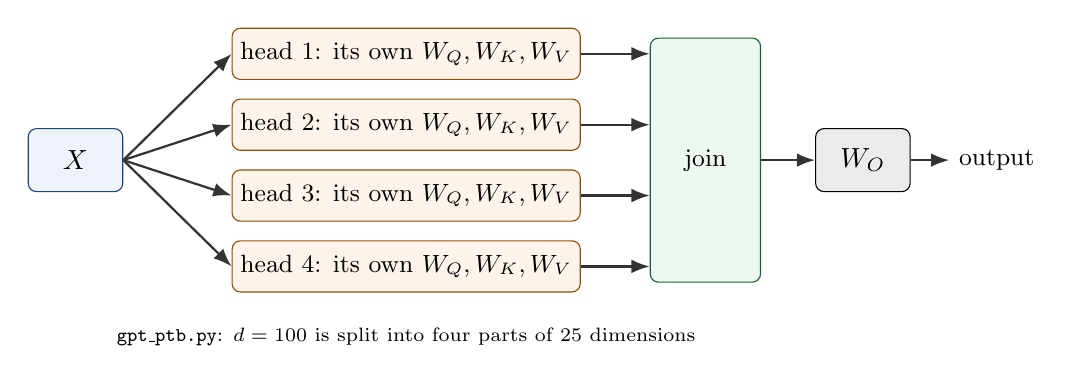
\begin{tikzpicture}[x=1cm,y=1cm]
\node[lay=tokc,minimum width=12mm] (x) at (0,0) {$X$};
\foreach \k/\y in {1/1.35,2/0.45,3/-0.45,4/-1.35}{
  \node[lay=attc,minimum width=40mm,minimum height=6.5mm,font=\small] (h\k) at (4.2,\y)
    {head \k: its own $W_Q,W_K,W_V$};
  \draw[ar] (x.east) -- (h\k.west);
}
\node[lay=grnc,minimum width=14mm,minimum height=31mm,font=\small] (cat) at (8.0,0) {join};
\foreach \k in {1,...,4} \draw[ar] (h\k.east) -- (h\k.east-|cat.west);
\node[lay,minimum width=12mm] (wo) at (10.0,0) {$W_O$};
\draw[ar] (cat) -- (wo);
\node[font=\small] (o) at (11.7,0) {output};
\draw[ar] (wo) -- (o);
\node[font=\scriptsize,align=center] at (4.2,-2.25)
  {\texttt{gpt\_ptb.py}: $d=100$ is split into four parts of $25$ dimensions};
\end{tikzpicture}
\end{adjustbox}
\figcap{head마다 어텐션을 따로 계산하고, 결과를 이어 붙여 $W_O$에 넣는다.}
\end{frame}

\subsection{Transformer의 구조}

\begin{frame}{Transformer의 구조}
\begin{columns}[c,onlytextwidth]
\begin{column}{0.6\textwidth}
\sfig[6.6cm]{transformer}
\end{column}
\begin{column}{0.38\textwidth}
\small
Encoder와 Decoder는 같은 모양의 블록을 $N$번 쌓은 것이다.
회색 화살표는 residual 연결이다.
\vskip3mm
\textbf{Encoder 블록}: self-attention (원문의 단어들이 서로를 본다) $\to$ Feed Forward
\vskip3mm
\textbf{Decoder 블록}: causal mask를 쓴 self-attention (번역문의 앞 단어들끼리)
$\to$ Encoder의 출력을 보는 어텐션 (9절과 같다: query는 Decoder, key와 value는 Encoder)
$\to$ Feed Forward
\end{column}
\end{columns}
\end{frame}

\begin{frame}{블록의 나머지 부품: Feed Forward와 add \& norm}
\begin{itemize}
\item \textbf{Feed Forward}: 은닉층이 하나인 신경망 (Linear $\to$ ReLU $\to$ Linear).
  모든 위치에 같은 가중치로 \textbf{따로} 적용된다.
  어텐션이 다른 위치에서 모아 온 정보를 위치마다 가공한다.
\item \textbf{add \& norm}: 각 부분의 출력을 입력에 \textbf{더하고} (residual 연결) 정규화한다.
\item \textbf{LayerNorm}: 벡터 하나의 성분들을 평균 $0$, 분산 $1$로 맞춘다.
  예: $(1,2,3,6)$은 평균 $3$, 분산 $3.5$이므로 $(-1.069,\ -0.5345,\ 0,\ 1.6036)$이 된다
  (\texttt{lm\_tiny.py}의 4번 셀).
\end{itemize}
\vskip1mm
\begin{keybox}[층을 깊게 쌓아도 학습이 되는 이유]
residual 연결은 CNN 단원의 ResNet, 7절의 LSTM 기억 셀과 같은 원리로 gradient를 잘 전달한다.
정규화는 각 층의 입력 크기를 일정하게 유지한다.
\end{keybox}
\vskip1mm
RNN이 없으므로 문장의 모든 위치를 동시에 계산한다.
큰 GPU에서 훨씬 많은 데이터로 학습할 수 있고, 번역 품질도 RNN 기반의 GNMT보다 좋았다.
\end{frame}

% =================================================
\section{GPT: Transformer로 만든 언어모델}
% =================================================

\subsection{Decoder 블록만 쌓는다}

\begin{frame}{Decoder 블록만 쌓는다}
\begin{itemize}
\item Transformer는 번역을 위해 만들어졌다.
  원문을 읽는 Encoder와 번역문을 쓰는 Decoder가 있다.
\item 5절의 언어모델은 앞의 단어들로 다음 단어를 맞힌다.
  원문이 따로 없으므로 \textbf{Encoder가 필요 없다}.
\item Decoder 블록에서 Encoder를 보는 어텐션을 빼면
  causal mask를 쓴 self-attention과 Feed Forward가 남는다.
\end{itemize}
\vskip3mm
\begin{keybox}
이 블록만 쌓아 만든 언어모델이 \textbf{GPT} (generative pre-trained transformer)이다
(Radford et al., 2018).
\end{keybox}
\end{frame}

\begin{frame}{GPT의 구조}
\begin{columns}[c,onlytextwidth]
\begin{column}{0.6\textwidth}
\sfig[6.6cm]{gpt}
\end{column}
\begin{column}{0.38\textwidth}
\small
\begin{itemize}
\item 단어 벡터에 위치 벡터를 더해 블록 $N$개에 넣는다.
\item 마지막 Linear 층이 \textbf{모든 위치에서} 다음 단어의 점수를 낸다.
\item 입력과 정답은 RNN 언어모델과 똑같다.
  정답은 입력을 한 칸 민 단어 열이고, loss도 같은 cross-entropy이다.
\item 다른 것은 가운데, 곧 \textbf{앞의 단어들을 보는 방법}이다.
\end{itemize}
\end{column}
\end{columns}
\end{frame}

\begin{frame}{RNN 언어모델과 GPT}
\begin{center}
\small
\begin{tabular}{@{}p{24mm}p{54mm}p{54mm}@{}}
\toprule
& RNN, LSTM 언어모델 & GPT \\
\midrule
앞의 단어를\newline 보는 방법 & 은닉 상태 하나에 요약해 둔다 & 어텐션으로 앞의 단어 벡터를 직접 본다 \\
계산 & 한 단어씩 순서대로 & 모든 위치를 동시에 \\
순서 정보 & 읽는 순서 & 위치 벡터 \\
볼 수 있는 범위 & 제한이 없지만 먼 단어는 흐려진다 & 정해진 길이 $T$까지 \\
\bottomrule
\end{tabular}
\end{center}
\vskip3mm
GPT가 한 번에 볼 수 있는 길이 $T$를 \textbf{context length}라 한다.
위치 벡터를 $T$개만 가지고 있기 때문이다.
\end{frame}

\subsection{PyTorch로 구현하기}

\begin{frame}[fragile]{PyTorch: self-attention 계층 (1) 준비}
\texttt{gpt\_ptb.py}의 2번 셀. \texttt{T}는 파일 앞에서 정한 context length ($64$)이다.
\begin{lstlisting}
class SelfAttention(nn.Module):
    def __init__(self, d, n_head):
        super().__init__()
        self.n_head = n_head
        self.W_Q, self.W_K, self.W_V = nn.Linear(d, d), nn.Linear(d, d), nn.Linear(d, d)
        self.W_O = nn.Linear(d, d)               # applied after the heads are joined
        future = torch.triu(torch.ones(T, T, dtype=torch.bool), diagonal=1)
        self.register_buffer("future", future)   # future[i, j] is True where j > i
\end{lstlisting}
\begin{itemize}
\item $W_Q$, $W_K$, $W_V$: $d$차원 벡터를 $d$차원으로 보내는 Linear 층.
  $W_O$는 head들의 결과를 이어 붙인 뒤에 쓴다.
\item \texttt{future}: 대각선 위 ($j>i$)만 \texttt{True}인 $T\times T$ 행렬. causal mask에 쓴다.
\item \texttt{register\_buffer}: 학습되는 가중치는 아니지만 모델과 함께 GPU로 옮겨진다.
\end{itemize}
\end{frame}

\begin{frame}[fragile]{PyTorch: self-attention 계층 (2) 계산}
\begin{lstlisting}
    def forward(self, x):                        # x: (B, T, d)
        B, T, d = x.shape
        # split every vector into n_head parts: (B, T, d) -> (B, heads, T, d/heads)
        split = lambda z: z.view(B, T, self.n_head, -1).transpose(1, 2)
        q, k, v = split(self.W_Q(x)), split(self.W_K(x)), split(self.W_V(x))
        S = q @ k.transpose(-2, -1) / math.sqrt(q.size(-1))      # scores q_i . k_j
        S = S.masked_fill(self.future[:T, :T], float("-inf"))    # causal mask
        A = torch.softmax(S, dim=-1)             # (B, heads, T, T), each row sums to 1
        O = (A @ v).transpose(1, 2).reshape(B, T, d)             # heads joined again
        return self.W_O(O)
\end{lstlisting}
\begin{itemize}
\item \texttt{q, k, v}부터 \texttt{O}까지 다섯 줄이 $O=\softmax(QK\T/\sqrt d)\,V$이다.
\item \texttt{masked\_fill}이 causal mask이다.
  \texttt{future}가 \texttt{True}인 곳, 곧 대각선 위의 점수를 $-\infty$로 바꾼다.
\item head가 $4$개이므로 $100$차원 벡터를 $25$차원 네 조각으로 나누어 조각마다 어텐션을
  계산하고, 결과를 다시 이어 붙인다. 그래서 점수를 $\sqrt{25}$로 나눈다.
\end{itemize}
\end{frame}

\begin{frame}[fragile]{PyTorch: 블록}
\begin{lstlisting}
class Block(nn.Module):
    def __init__(self, d, n_head):
        super().__init__()
        self.attn = SelfAttention(d, n_head)
        self.ff = nn.Sequential(nn.Linear(d, 4 * d), nn.ReLU(), nn.Linear(4 * d, d))
        self.norm1, self.norm2 = nn.LayerNorm(d), nn.LayerNorm(d)

    def forward(self, x):
        x = self.norm1(x + self.attn(x))         # masked self-attention, add & norm
        x = self.norm2(x + self.ff(x))           # feed forward, add & norm
        return x
\end{lstlisting}
\begin{itemize}
\item \texttt{forward}의 두 줄이 GPT 그림의 블록 하나이다.
  더하고 (residual 연결) 정규화하기를 두 번 한다.
\item Feed Forward는 $d\to4d\to d$이다. 모든 위치에 같은 가중치로 따로 적용된다.
\end{itemize}
\end{frame}

\begin{frame}[fragile]{PyTorch: GPT 모델}
\begin{lstlisting}
class GPT(nn.Module):
    def __init__(self, V, d=100, n_head=4, n_layer=2):
        super().__init__()
        self.tok = nn.Embedding(V, d)            # word ID  -> vector
        self.pos = nn.Embedding(T, d)            # position -> vector
        self.blocks = nn.Sequential(*[Block(d, n_head) for _ in range(n_layer)])
        self.out = nn.Linear(d, V)

    def forward(self, x):                        # x: (B, T) word IDs
        h = self.tok(x) + self.pos(torch.arange(x.size(1), device=x.device))  # (B, T, d)
        return self.out(self.blocks(h))          # (B, T, V): scores of the next word
\end{lstlisting}
\begin{itemize}
\item 단어 벡터와 위치 벡터를 더해 블록들에 넣는다.
  위치 벡터는 학습되는 \texttt{nn.Embedding(T, d)}이다.
\item 출력의 shape은 $(B,T,V)$로, RNN 언어모델과 같다.
\end{itemize}
\end{frame}

\begin{frame}{지금의 언어모델은 블록을 조금 다르게 만든다}
\texttt{gpt\_ptb.py}의 블록은 처음 Transformer 논문의 모양 (더한 뒤 정규화, post-norm)이다.
수십--수백 층을 쌓는 지금의 언어모델은 몇 군데를 바꾸었다.
뼈대 (어텐션, Feed Forward, residual 연결, 정규화)는 같다.
\vskip1mm
\begin{center}
\footnotesize
\begin{tabular}{@{}p{24mm}p{36mm}p{75mm}@{}}
\toprule
바뀐 곳 & 지금의 언어모델 & 효과 \\
\midrule
정규화의 위치 & pre-norm (정규화한 뒤 더한다)
  & residual 연결의 길에 정규화가 끼지 않아 gradient가 깊은 층까지 그대로 전달된다
  (GPT-2부터) \\
정규화 & RMSNorm & 평균을 빼지 않고 크기만 맞춘다. 계산이 가볍다 \\
활성화 함수 & GELU, SwiGLU & SwiGLU는 게이트를 곱하는 형태 (LSTM의 게이트와 비슷한 생각) \\
위치 정보 & RoPE & 학습 때보다 긴 글에도 비교적 잘 늘어난다 \\
key와 value & grouped-query attention
  & 여러 query head가 key, value head 하나를 함께 쓴다. KV cache의 메모리가 준다 \\
Feed Forward & mixture of experts (MoE)
  & 여러 개 가운데 토큰마다 몇 개만 골라 쓴다. 가중치는 많아도 토큰 하나의 계산은 적다 \\
\bottomrule
\end{tabular}
\end{center}
\end{frame}

\begin{frame}{가중치 수}
어휘 $V=10{,}000$, $d=100$, 블록 $2$개, $T=64$일 때 가중치는 모두 $2{,}259{,}000$개이다.
\begin{center}
\begin{tabular}{@{}llr@{}}
\toprule
부분 & 계산 & 가중치 수 \\
\midrule
단어 Embedding & $10{,}000\times100$ & $1{,}000{,}000$ \\
위치 Embedding & $64\times100$ & $6{,}400$ \\
블록 $2$개 & $2\times121{,}300$ & $242{,}600$ \\
출력층 & $100\times10{,}000+10{,}000$ & $1{,}010{,}000$ \\
\bottomrule
\end{tabular}
\end{center}
\begin{itemize}
\item 블록 하나의 $121{,}300$개: 어텐션의 Linear 네 개 ($4\times10{,}100$),
  Feed Forward ($40{,}400+40{,}100$), LayerNorm 두 개 ($2\times200$).
\item 가중치의 대부분은 단어 Embedding과 출력층에 있다.
  7절의 LSTM 언어모델 ($2{,}090{,}800$개)도 마찬가지로, LSTM 계층의 가중치는 $80{,}800$개뿐이다.
\end{itemize}
\end{frame}

\subsection{PTB로 학습하기: RNN, LSTM과 비교}

\begin{frame}{PTB로 학습하기}
7절과 같은 PTB를 같은 설정 (벡터 $100$차원, Adam, 학습률 $10^{-3}$, gradient clipping,
$10$ epoch)으로 학습한다 (\texttt{gpt\_ptb.py}). 블록 $2$개, head $4$개, $T=64$.
\vskip2mm
미니배치를 만드는 방법만 다르다.
\vskip1mm
\begin{columns}[T,onlytextwidth]
\begin{column}{0.48\textwidth}
\begin{remarkbox}[RNN, LSTM]
은닉 상태를 이어 가야 하므로 말뭉치를 \textbf{순서대로} 읽는다.
\end{remarkbox}
\end{column}
\begin{column}{0.48\textwidth}
\begin{keybox}[GPT]
이어 갈 상태가 없으므로 말뭉치의 \textbf{아무 곳에서나} 길이 $64$의 조각 $20$개를 뽑는다.
\end{keybox}
\end{column}
\end{columns}
\vskip2mm
조각 하나의 $64$개 위치가 모두 학습 예이다.
loss는 $20\times64=1{,}280$개 위치의 cross-entropy의 평균이다.
\end{frame}

\begin{frame}{결과: 퍼플렉서티}
\begin{columns}[c,onlytextwidth]
\begin{column}{0.48\textwidth}
\pfig[4.7cm]{figures/gpt_ppl.png}
\figcap{epoch마다 잰 검증 퍼플렉서티. RNN과 LSTM은 7절의 결과이다.}
\end{column}
\begin{column}{0.49\textwidth}
\small
\begin{tabular}{@{}lccc@{}}
\toprule
모델 & 가중치 수 & 검증 & 테스트 \\
\midrule
RNN & $2{,}030{,}200$ & $172.8$ & $161.9$ \\
LSTM & $2{,}090{,}800$ & $156.1$ & $144.3$ \\
GPT & $2{,}259{,}000$ & $151.3$ & $139.7$ \\
\bottomrule
\end{tabular}
\vskip1mm
{\footnotesize $10$ epoch 후의 퍼플렉서티\par}
\end{column}
\end{columns}
\end{frame}

\begin{frame}{결과 읽기}
\begin{itemize}
\item GPT의 퍼플렉서티가 가장 낮다.
  다만 LSTM과의 차이는 작고 ($144.3$과 $139.7$), 가중치는 GPT가 조금 더 많다.
\item RNN과 LSTM은 은닉 상태를 통해 글의 처음부터 이어서 읽는다.
  GPT는 각 단어를 앞의 $33$--$64$단어만 보고 맞혔다 (\texttt{gpt\_ptb.py}의 3번 셀).
  그런데도 퍼플렉서티가 더 낮다.
\item 이 크기에서 GPT의 학습이 LSTM보다 빠르지는 않다.
  RTX 3050에서 세 모델 모두 $10$ epoch에 몇 분이 걸린다.
\item 모든 위치를 동시에 계산하는 이점은 모델과 데이터가 클 때 나타난다.
\end{itemize}
\end{frame}

\begin{frame}{글 이어 쓰기}
생성 방법은 8절과 같다 (\texttt{gpt\_ptb.py}의 5번 셀).
\begin{enumerate}
\item 지금까지의 글 (최대 $T$단어)을 넣는다.
\item 마지막 위치의 점수에서 다음 단어를 뽑는다.
\item 뽑은 단어를 뒤에 붙이고 1로 돌아간다.
\end{enumerate}
\vskip2mm
\begin{remarkbox}[RNN과 다른 점]
RNN은 은닉 상태가 있어 새 단어 하나만 넣으면 되었다.
GPT는 상태가 없으므로 매번 글 전체를 다시 넣는다.
그러면 앞 위치들의 계산을 매번 되풀이한다.
\end{remarkbox}
\end{frame}

\begin{frame}{KV cache}
causal mask 때문에 앞 위치의 출력은 뒤에 붙는 단어의 영향을 받지 않는다.
새 단어에게 필요한 것은 앞 위치들의 \textbf{key와 value}뿐이다.
\begin{itemize}
\item 블록마다 앞 위치의 key와 value를 저장해 두고 (KV cache),
  새 단어 하나의 query, key, value만 계산한다.
\item 새 query와 저장된 key들의 내적이 점수이고, 그 가중치로 저장된 value들을 가중합한다:
  \ $s_j=\vect q_n\cdot\vect k_j/\sqrt d$ ($j=1,\dots,n$),\ \ $\vect o_n=\sum_j a_j\vect v_j$.
\item $n$번째 단어를 만들 때 한 head의 점수 계산이 약 $n^2/2$번에서 $n$번으로 줄어든다.
  대신 저장할 메모리가 글의 길이에 비례해 늘어난다.
  긴 대화에서 언어모델이 메모리를 많이 쓰는 큰 이유이다.
\end{itemize}
\begin{keybox}
KV cache는 RNN의 은닉 상태와 같은 역할을 한다.
RNN은 크기가 고정된 벡터 하나에 요약하고, GPT는 앞 위치의 key와 value를 모두 남겨 둔다.
\end{keybox}
\end{frame}

\begin{frame}{GPT가 이어 쓴 글}
\begin{remarkbox}[GPT가 이어 쓴 글 (밑줄이 prompt)]
\ttfamily\footnotesize\raggedright
\textsf{$\tau=0.5$:} \underline{the company said it} expects to report the full fiscal N revenue
of \$ N million to \$ N million from \$ N million / the company said its\\[0.6em]
\textsf{$\tau=1.0$:} \underline{the company said it} expects to drop the full fiscal federal
conduct a merger of c\$ N million while will rise N N to N N including N million\\[0.6em]
\textsf{$\tau=1.5$:} \underline{the company said it} expects more accrued higher somewhere /
federal conduct a merger warning bullets to ownership of drugs however fannie losses widened
from free tuesday found our
\end{remarkbox}
\vskip2mm
LSTM의 글과 마찬가지로 $\tau$가 작을수록 무난한 구절이 이어지고, $\tau$가 크면 문법이 무너진다.
(PTB는 숫자를 \w{N}으로, 드문 단어를 \w{<unk>}로 바꾸어 두었다.)
\end{frame}

\subsection{word2vec에서 Transformer로: 고정된 표현과 문맥 표현}

\begin{frame}{고정된 표현과 문맥 표현}
3--4절의 word2vec과 Transformer는 어떤 관계일까?
둘 다 단어를 밀집 벡터로 나타낸다.
차이는 \textbf{그 벡터가 문맥에 따라 달라지는가}이다.
\vskip2mm
\sfig[4.0cm]{static_vs_context}
\figcap{word2vec은 문장과 상관없이 같은 벡터를, Transformer는 문맥에 따라 다른 벡터를 준다.}
\end{frame}

\begin{frame}{단어마다 벡터 하나, 위치마다 벡터 하나}
\begin{itemize}
\item \textbf{word2vec: 단어마다 벡터 하나.}
  \w{the river bank} (강둑)의 \w{bank}와 \w{a bank account} (은행)의 \w{bank}가 같은 벡터이다.
  여러 뜻이 한 벡터에 섞인다.
\item \textbf{Transformer: 문장 속 위치마다 벡터 하나.}
  첫 층의 Embedding에서는 고정된 벡터로 시작하지만, 층을 지날 때마다 self-attention으로
  \w{river} 또는 \w{account}의 정보가 더해진다.
  마지막 층에서 \w{bank}의 벡터는 문장마다 다르다.
  이것을 \textbf{문맥 표현} (contextual representation)이라 한다.
\end{itemize}
\vskip3mm
\begin{keybox}[공통점]
둘 다 \textbf{글에서 단어를 맞히는 예측을 학습하다 보니} 단어의 의미가 벡터에 담긴다
(1절의 분포 가설).
GPT는 word2vec의 생각을 맥락은 훨씬 길게, 모델은 훨씬 크게 키운 것이라고 볼 수 있다.
\end{keybox}
\end{frame}

\begin{frame}{word2vec과 Transformer}
\begin{center}
\small
\begin{tabular}{@{}lll@{}}
\toprule
& word2vec & Transformer (GPT 등) \\
\midrule
벡터의 수 & 단어마다 하나, 고정 & 문장 속 위치마다 하나, 문맥에 따라 다름 \\
보는 맥락 & 좌우 몇 단어 (평균) & 문장 전체 (attention) \\
학습 & 맥락으로 가운데 단어 맞히기 & 앞의 글로 다음 토큰 맞히기 \\
벡터의 역할 & 그 자체가 결과물 & 다음 토큰을 맞히기 위한 중간 표현 \\
\bottomrule
\end{tabular}
\end{center}
\vskip3mm
``글을 벡터로 바꾸어 비슷한 것을 찾는다''는 word2vec의 쓰임도 그대로 남아 있다.
\begin{itemize}
\item 검색, 추천, 그리고 언어모델이 관련 문서를 찾아 답하는 방법 (RAG)에서는
  Transformer로 문장이나 문서 전체를 벡터 하나로 바꾸는 \textbf{임베딩 모델}을 쓴다.
\item 비슷한 문서를 찾을 때는 2절과 똑같이 코사인 유사도를 계산한다.
\end{itemize}
\end{frame}

\subsection{토큰: 단어보다 작은 조각}

\begin{frame}{단어를 단위로 쓰면 불편한 점}
\begin{itemize}
\item 어휘를 미리 정해야 한다.
  PTB는 흔한 단어 $10{,}000$개만 남기고 나머지를 모두 \w{<unk>}로 바꾸어 둔 것이다.
  어휘에 없는 단어는 읽지도 쓰지도 못한다.
\item \w{walk}, \w{walks}, \w{walked}, \w{walking}이 서로 관계없는 네 단어가 된다.
\end{itemize}
\vskip1mm
글자를 단위로 쓰면 모르는 단어는 없어진다.
대신 글이 길어지고, 글자 하나에는 뜻이 거의 없다.
\vskip2mm
\begin{keybox}[토큰]
지금의 언어모델은 그 중간인 \textbf{단어 조각}을 단위로 쓴다.
이 단위를 \textbf{토큰} (token)이라 한다.
흔한 단어는 통째로 토큰 하나가 되고, 드문 단어는 몇 개의 조각으로 나뉜다.
\end{keybox}
\end{frame}

\begin{frame}{BPE: 자주 이웃하는 쌍을 합친다}
토큰을 정하는 대표적인 방법이 \textbf{BPE} (byte pair encoding)이다.
\begin{enumerate}
\item 모든 단어를 글자로 쪼갠다. 단어의 끝에는 끝 표시 (\w{\_})를 붙인다.
\item 말뭉치에서 가장 자주 이웃해 나오는 토큰 두 개를 찾아 새 토큰 하나로 합친다.
\item 정해 둔 횟수만큼 2를 반복한다.
\end{enumerate}
\vskip2mm
\begin{itemize}
\item BPE는 \textbf{세기만} 한다. 신경망이 아니고 학습되는 가중치도 없다.
  언어모델을 학습하기 전에 한 번 만들어 두는 규칙이다.
\item 언어모델 쪽에서 달라지는 것은 Embedding의 행이 단어가 아니라 토큰에 대응한다는 것뿐이다.
  모델은 다음 \textbf{토큰}을 맞힌다.
\end{itemize}
\end{frame}

\begin{frame}{BPE의 작은 예}
\w{low}가 $5$번, \w{lower}가 $2$번, \w{newest}가 $6$번, \w{widest}가 $3$번 나오는 말뭉치에서
여덟 번 합친다 (\texttt{bpe\_tokens.py}의 2번 셀).
\begin{center}
\ttfamily\footnotesize
\begin{tabular}{@{}cll@{}}
\toprule
\sffamily 합치기 & \sffamily 합친 쌍 (나온 횟수) & \sffamily 말뭉치의 네 단어 \\
\midrule
& & l o w \_ \quad l o w e r \_ \quad n e w e s t \_ \quad w i d e s t \_ \\
1 & t $+$ \_ \ (9) & l o w \_ \quad l o w e r \_ \quad n e w e s t\_ \quad w i d e s t\_ \\
2 & s $+$ t\_ \ (9) & l o w \_ \quad l o w e r \_ \quad n e w e st\_ \quad w i d e st\_ \\
3 & e $+$ st\_ \ (9) & l o w \_ \quad l o w e r \_ \quad n e w est\_ \quad w i d est\_ \\
4 & o $+$ w \ (7) & l ow \_ \quad l ow e r \_ \quad n e w est\_ \quad w i d est\_ \\
5 & l $+$ ow \ (7) & low \_ \quad low e r \_ \quad n e w est\_ \quad w i d est\_ \\
6 & w $+$ est\_ \ (6) & low \_ \quad low e r \_ \quad n e west\_ \quad w i d est\_ \\
7 & n $+$ e \ (6) & low \_ \quad low e r \_ \quad ne west\_ \quad w i d est\_ \\
8 & ne $+$ west\_ \ (6) & low \_ \quad low e r \_ \quad newest\_ \quad w i d est\_ \\
\bottomrule
\end{tabular}
\end{center}
\w{newest}와 \w{widest}에 함께 나오는 \w{est\_}, \w{low}와 \w{lower}에 함께 나오는 \w{low}가
토큰이 되었다.
말뭉치에 없던 단어 \w{lowest}는 \w{low} \w{est\_}, 곧 아는 토큰 두 개가 된다.
\end{frame}

\begin{frame}{PTB에 BPE 적용하기}
PTB의 학습 데이터 (\w{<unk>}를 뺀 $842{,}501$단어, 서로 다른 단어 $9{,}998$개)의 글자는
끝 표시까지 $47$종이다.
$1{,}000$번 합치면 토큰은 $1{,}047$종이 된다 (\texttt{bpe\_tokens.py}의 3, 4번 셀).
\begin{columns}[c,onlytextwidth]
\begin{column}{0.58\textwidth}
\begin{center}
\small
\begin{tabular}{@{}lrl@{}}
\toprule
단어 & 나온 횟수 & 토큰 \\
\midrule
\w{the} & $50{,}770$ & \w{the\_} \\
\w{company} & $2{,}680$ & \w{company\_} \\
\w{international} & $467$ & \w{international\_} \\
\w{toyota} & $30$ & \w{to}\ \ \w{y}\ \ \w{o}\ \ \w{t}\ \ \w{a\_} \\
\w{galvanized} & $11$ & \w{g}\ \ \w{al}\ \ \w{v}\ \ \w{an}\ \ \w{iz}\ \ \w{ed\_} \\
\w{unbelievable} & $0$ & \w{un}\ \ \w{be}\ \ \w{li}\ \ \w{ev}\ \ \w{able\_} \\
\w{tokenization} & $0$ & \w{to}\ \ \w{k}\ \ \w{en}\ \ \w{iz}\ \ \w{ation\_} \\
\w{chatgpt} & $0$ & \w{ch}\ \ \w{at}\ \ \w{g}\ \ \w{pt\_} \\
\bottomrule
\end{tabular}
\end{center}
\end{column}
\begin{column}{0.39\textwidth}
처음 합쳐지는 쌍은 \w{e}$+$\w{\_}, \w{s}$+$\w{\_}, \w{t}$+$\w{h}, \w{i}$+$\w{n}이고,
열 번째에 \w{th}$+$\w{e\_}가 합쳐져 \w{the\_}가 토큰이 된다.
\vskip2mm
흔한 단어는 토큰 하나, 드문 단어는 여러 조각이다.
말뭉치에 없던 단어도 아는 조각으로 쓸 수 있다.
\end{column}
\end{columns}
\end{frame}

\begin{frame}{토큰으로 무엇이 좋아졌나}
\begin{itemize}
\item 흔한 단어는 토큰 하나이고 ($9{,}998$개 중 $327$개), 드문 단어는 여러 조각으로 나뉜다.
  말뭉치에 없던 단어도 조각으로 쓸 수 있으므로 \w{<unk>}가 필요 없다.
\item 글자로 쓰면 단어 하나가 평균 $5.63$개 (끝 표시 포함), 이 토큰으로 쓰면 평균 $1.76$개이다.
  어휘는 단어 단위 ($10{,}000$)의 약 $1/10$인데 글은 $1.76$배 길어질 뿐이다.
\item 실제 GPT는 글자 대신 byte에서 시작하므로 한글이나 기호도 모두 나타낼 수 있다.
  GPT-2와 GPT-3의 어휘는 토큰 $50{,}257$개이다.
\item 언어모델의 context length와 사용 요금을 토큰 수로 세는 것은
  토큰이 모델이 다루는 단위이기 때문이다.
\end{itemize}
\end{frame}

\subsection{작은 GPT에서 대화형 언어모델로}

\begin{frame}{Encoder만 쓰는 모델, Decoder만 쓰는 모델}
Transformer의 Encoder와 Decoder는 따로 발전했다.
\vskip1mm
\begin{columns}[T,onlytextwidth]
\begin{column}{0.48\textwidth}
\begin{remarkbox}[Encoder만 쓰는 모델: BERT 등]
\small
\begin{itemize}
\item causal mask 없이 문장 전체를 양쪽에서 본다.
\item 글을 이어 쓰지는 못한다. 분류나 검색에 쓴다.
\item 단어 몇 개를 가리고 양쪽 맥락으로 맞히게 학습한다 (3절의 CBOW와 닮았다).
\end{itemize}
\end{remarkbox}
\end{column}
\begin{column}{0.48\textwidth}
\begin{keybox}[Decoder만 쓰는 모델: GPT 등]
\small
\begin{itemize}
\item 이 절에서 만든 모델이다.
\item 앞의 토큰들로 다음 토큰을 맞히며 학습한다.
\item 한 토큰씩 뽑아 글을 이어 쓴다.
\end{itemize}
\end{keybox}
\end{column}
\end{columns}
\vskip2mm
ChatGPT 같은 대화형 언어모델은 두 번째이다.
\texttt{gpt\_ptb.py}의 모델과 구조가 같고, 다른 것은 \textbf{크기}와 \textbf{학습 단계}이다.
\end{frame}

\begin{frame}{크기: \texttt{gpt\_ptb.py}와 GPT-3}
구조가 논문으로 공개된 GPT-3 (2020년)와 비교하면 다음과 같다.
\begin{center}
\begin{tabular}{@{}lrr@{}}
\toprule
& \texttt{gpt\_ptb.py} & GPT-3 \\
\midrule
가중치 수 & $226$만 & $1{,}750$억 \\
블록 수 $N$ & $2$ & $96$ \\
벡터의 차원 $d$ & $100$ & $12{,}288$ \\
head 수 & $4$ & $96$ \\
context length & 단어 $64$개 & 토큰 $2{,}048$개 \\
어휘 & 단어 $10{,}000$개 & 토큰 $50{,}257$개 \\
학습에 쓴 글 & 단어 $93$만 개 & 토큰 약 $3{,}000$억 개 \\
\bottomrule
\end{tabular}
\end{center}
\end{frame}

\begin{frame}{크게 만들면 좋아진다: 스케일링 법칙}
\begin{itemize}
\item 가중치 수, 학습에 쓴 토큰 수, 계산량을 늘리면 테스트 loss가 \textbf{거듭제곱 법칙}을 따라
  꾸준히 줄어든다는 것이 실험으로 알려졌다 (Kaplan et al., 2020).
\item 모델 구조를 새로 고안하지 않아도 크기만 키우면 예측 가능하게 좋아진다는 뜻이다.
  이것이 언어모델이 빠르게 커진 이유이다.
\item 그 뒤 같은 계산량이면 모델만 키우기보다 데이터도 함께 늘리는 것이 낫다는 결과
  (가중치 하나에 토큰 약 $20$개; Hoffmann et al., 2022)가 나왔다.
  지금은 그보다 훨씬 많은 토큰으로 학습하는 경우가 많다.
\end{itemize}
\vskip2mm
\begin{remarkbox}[이 단원의 실험도 같은 방향을 보인다]
PTB의 $93$만 단어로는 \w{king}--\w{queen}을 풀지 못했고 (4절),
작은 GPT의 퍼플렉서티도 $140$ 근처였다.
\end{remarkbox}
\end{frame}

\begin{frame}{학습 단계}
\small
사전학습만 한 모델은 글을 이어 쓸 뿐, 질문에 답하지 않는다.
``한국의 수도는?''을 주면 답 대신 비슷한 질문을 몇 개 더 이어 쓸 수도 있다.
\begin{enumerate}
\item \textbf{사전학습} (pre-training): 많은 글로 다음 토큰 맞히기를 학습한다. GPT의 P가 이것이다.
  계산의 대부분이 여기에 들고, 언어와 지식은 주로 이 단계에서 배운다.
\item \textbf{지시 학습} (instruction tuning, supervised fine-tuning):
  질문 (지시)과 좋은 답을 사람이 써 둔 예로 더 학습한다.
  loss는 그대로 다음 토큰의 cross-entropy이고, 데이터만 다르다.
\item \textbf{선호 학습} (RLHF 등): 사람이 두 답을 비교해 고른 것을 흉내 내는
  점수 모델 (reward model)을 학습하고, 그 점수가 높은 답을 내도록 강화학습으로 조정한다
  (InstructGPT, ChatGPT, 2022년). 점수 모델 없이 비교 데이터로 바로 학습하는 DPO도 많이 쓴다.
\end{enumerate}
\vskip1mm
\begin{keybox}
대화도 글 이어 쓰기이다. 대화는 \w{<user>} 질문 \w{<assistant>} 답 \dots\ 같은 특별한 토큰으로
구분한 하나의 긴 글이고, 사용자의 질문이 prompt, 모델이 그 뒤에 이어 쓴 글이 답이다.
\end{keybox}
\end{frame}

\begin{frame}{최근의 흐름 (1)}
구조는 이 단원의 Decoder 블록 그대로이고, 쓰는 방법이 넓어지고 있다.
\begin{itemize}
\item \textbf{prompt 안에서 배우기} (in-context learning): prompt에 예를 몇 개 보여 주면,
  가중치를 바꾸지 않고도 그 형식의 과제를 푼다 (GPT-3).
  답을 쓸 때 어텐션으로 prompt 안의 예를 참고할 수 있기 때문이다.
\item \textbf{답하기 전에 생각하기} (reasoning model): 답을 바로 쓰지 않고 풀이 과정을 길게
  먼저 써 내려가게 한다. 정답을 확인할 수 있는 문제 (수학 등)로 강화학습을 하여 이 능력을
  키운다 (2024년 이후). 토큰을 더 많이 쓰는 만큼 어려운 문제를 더 잘 푼다.
\item \textbf{긴 context}: context length가 GPT-3의 $2{,}048$토큰에서 수십만--백만 토큰으로 늘었다.
  RoPE를 늘리는 방법, 메모리를 적게 쓰는 어텐션 계산 (FlashAttention),
  KV cache를 줄이는 방법이 이것을 가능하게 했다.
\end{itemize}
\end{frame}

\begin{frame}{최근의 흐름 (2)와 남은 한계}
\begin{itemize}
\item \textbf{도구와 검색}: 모르는 것은 검색해서 (RAG), 계산은 코드를 실행해서 답한다.
  모델이 ``검색하라''는 토큰을 이어 쓰면 프로그램이 그것을 실행하고 결과를 다시 prompt에 붙여 준다.
  여러 단계를 스스로 계획하고 실행하는 것을 agent라 부른다.
\item \textbf{글 밖으로}: 그림을 작은 조각 (patch)으로 나누어 조각마다 벡터 하나로 만들면
  Transformer가 토큰처럼 읽는다 (Vision Transformer).
  그림, 소리를 함께 읽는 언어모델 (multimodal)은 이렇게 만든다.
\end{itemize}
\vskip2mm
\begin{thinkbox}[남은 한계]
다음 토큰을 그럴듯하게 맞히도록 학습했으므로, 사실이 아닌 내용을 자신 있게 쓰기도 한다
(hallucination). 검색으로 근거를 붙이거나 답을 검증하는 방법이 함께 쓰이는 이유이다.
\end{thinkbox}
\end{frame}

\subsection{단원 전체의 정리}

\begin{frame}{단원 전체의 정리: 문제와 해결}
각 주제는 앞의 방법의 문제를 하나씩 해결하며 나왔다.
\begin{center}
\small
\begin{tabular}{@{}p{64mm}p{58mm}l@{}}
\toprule
문제 & 해결 & 절 \\
\midrule
단어는 숫자가 아니다 & 맥락을 세어 만든 단어 벡터 & 1, 2 \\
큰 말뭉치에서는 세어 만든 행렬을 다루기 어렵다 & 맞히면서 배운다: word2vec & 3, 4 \\
문장은 길이가 제각각이고 순서가 있다 & 은닉 상태로 요약하며 읽는다: RNN & 5, 6 \\
먼 단어의 gradient가 사라진다 & 기억 셀과 게이트: LSTM & 7 \\
문장을 받아 문장을 내야 한다 & Encoder와 Decoder: seq2seq & 8 \\
벡터 하나에 긴 문장을 담지 못한다 & 필요한 곳을 골라 본다: 어텐션 & 9 \\
RNN은 한 단어씩 순서대로 계산한다 & 어텐션만 쓴다: Transformer & 10 \\
어휘에 없는 단어를 다루지 못한다 & 단어 조각: 토큰 & 11 \\
\bottomrule
\end{tabular}
\end{center}
\end{frame}

\begin{frame}{바뀌지 않은 것}
\begin{keybox}
\textbf{글의 일부를 가리고 맞히게 하면, 맞히는 데 필요한 것을 신경망이 스스로 배운다.}
\end{keybox}
\vskip2mm
\begin{itemize}
\item word2vec은 가운데 단어를, RNN과 GPT는 다음 단어를 맞혔다.
\item 지금의 언어모델은 이 방법을 큰 Transformer와 많은 글에 적용한 것이다.
\end{itemize}
\end{frame}

\begin{frame}{9--11절 정리 (1)}
\begin{mlbox}[9--11절 정리]
\small
\begin{itemize}
\item seq2seq는 입력을 고정 길이 벡터 하나로 요약하므로 긴 문장에 약하다.
  어텐션은 Encoder의 모든 은닉 상태 $\vect{hs}$를 남겨 두고, Decoder가 매 시각 필요한 부분을
  골라 본다.
\item 고르기는 가중합으로 한다. 가중치는 Decoder의 은닉 상태와 $\vect{hs}$의 각 행의 내적에
  softmax를 취해 만든다.
\item 날짜 변환에서 어텐션은 출력의 각 부분에 해당하는 입력 부분을 스스로 찾아 본다.
\item Transformer는 RNN 없이 self-attention으로 만든다.
  query, key, value로 한 문장의 단어들이 서로를 보고, 위치 정보는 위치 벡터를 더해 넣는다.
  모든 위치를 동시에 계산하므로 큰 데이터로 학습할 수 있다.
\item Transformer의 블록은 어텐션, Feed Forward, 그리고 둘을 감싸는 residual 연결과
  LayerNorm으로 이루어진다.
\end{itemize}
\end{mlbox}
\end{frame}

\begin{frame}{9--11절 정리 (2)}
\begin{mlbox}[9--11절 정리]
\small
\begin{itemize}
\item causal mask를 쓴 블록만 쌓아 다음 단어 맞히기를 학습한 것이 GPT이다.
  입력, 정답, loss, 생성 방법은 RNN 언어모델과 같다.
\item word2vec의 단어 벡터는 고정되어 있고, Transformer의 벡터는 문맥에 따라 달라진다.
\item 지금의 언어모델은 단어 대신 토큰 (단어 조각)을 단위로 쓴다.
  BPE는 자주 이웃하는 쌍을 합쳐 토큰을 만든다.
\item 생성할 때는 앞 위치의 key와 value를 저장해 두고 (KV cache) 새 토큰만 계산한다.
  뽑는 방법은 temperature와 top-p로 조절한다.
\item 대화형 언어모델은 같은 구조를 크게 만들어 사전학습하고, 지시 학습과 선호 학습을 더한 것이다.
\end{itemize}
\end{mlbox}
\end{frame}

\end{document}
